\documentclass[tikz,border=12pt]{standalone}
\usepackage{amsmath}
\usetikzlibrary{arrows.meta}

\begin{document}
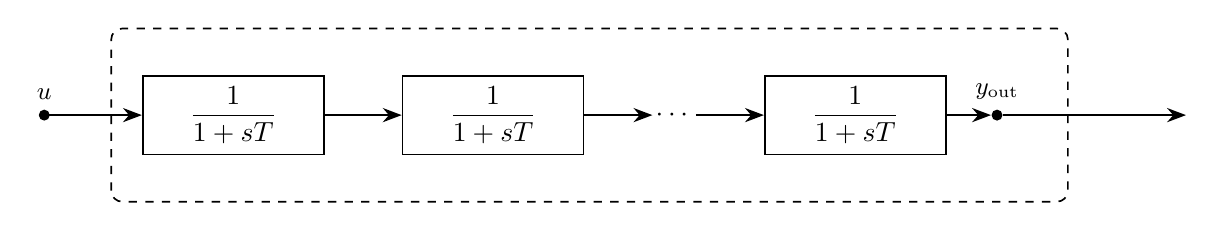
\begin{tikzpicture}[
    >={Stealth[length=2.4mm]},
    line/.style   = {semithick},
    block/.style  = {draw, semithick, fill=white,
                     minimum height=1cm, minimum width=2.3cm},
    signal/.style = {circle, fill, inner sep=1.4pt, label distance=3pt},
    sig/.style    = {font=\small}
]

% Lag-block chain: u -> 1/(1+sT) -> ... -> y_{N-1} = y_out
\foreach \k/\x in {0/0, 1/3.3, n/7.9}
    \node[block] (b\k) at (\x, 0) {$\dfrac{1}{1 + sT}$};
\node[inner sep=1pt] (dots) at (5.6, 0) {$\cdots$};

% input node (outside box)
\node[signal, label={[sig]above:$u$}] at (-2.4, 0) {};
\draw[->, line] (-2.4, 0) -- (b0.west);

% inter-block connections
\draw[->, line] (b0.east) -- (b1.west);
\draw[->, line] (b1.east) -- (dots);
\draw[->, line] (dots)    -- (bn.west);

% output node (inside box) with port arrow out
\node[signal, label={[sig]above:$y_{\mathrm{out}}$}] (yout) at (9.7, 0) {};
\draw[->, line] (bn.east) -- (yout);
\draw[->, line] (yout) -- (12.1, 0);

% model enclosure
\draw[dashed, semithick, rounded corners=4pt] (-1.55, -1.1) rectangle (10.6, 1.1);

\end{tikzpicture}
\end{document}
